\documentclass[11pt,oneside]{book}
\usepackage{graphicx}
\usepackage{booktabs}
\usepackage{caption}
\usepackage{subcaption}
\usepackage{amsmath}
\usepackage{amsfonts}
\usepackage{amssymb}
\usepackage{lscape}
\usepackage{psfrag}
\usepackage[usenames]{color}
\usepackage{bbm}
\usepackage[update]{epstopdf}
\usepackage[bookmarks,pdfstartview=FitH,a4paper,pdfborder={0 0 0}]{hyperref}
\usepackage{verbatim}
\usepackage{listings}
\usepackage{textcomp}
\usepackage{fancyhdr}
\usepackage{multirow}
\usepackage{tikz}
\usepackage{lipsum}
\usepackage{xcolor}
\usepackage[margin=1in]{geometry}
\newcommand{\hint}[1]{{\color{blue} \em #1}}

\usepackage{xspace}
\newcommand*{\eg}{e.g.\@\xspace}
\newcommand*{\ie}{i.e.\@\xspace}

\usepackage{xcolor, soul}
\usepackage[shortlabels]{enumitem}

\definecolor{GoodBlue}{rgb}{0.6640625,0.8203125,1}
\sethlcolor{GoodBlue}

\newcommand{\smallindent}{\hphantom{N}}
%\usepackage{appendix}
%\usepackage[title]{appendix}
\usepackage[titletoc]{appendix}

\begin{document}

% Update the Thesis information below!
\begin{titlepage}
    \centering
    
\includegraphics[width=\textwidth]{figures/eth-nsg-header}\\[60mm]
    %
    {\Huge\bf\sf{
        Advancing Packet-Level Traffic Predictions \\
        with Transformers  %\\[5mm]
        % Second Line of Thesis Title
    }}\\[10mm]
    {\Large\bf\sf Master Thesis}\\[3mm]
    %
    {\Large\bf\sf Author: Siddhant Ray } \\[5mm]
    {\sf Tutors: Alexander Dietmüller, Dr. Romain Jacob}\\[5mm]
    {\sf Supervisor: Prof. Dr. Laurent Vanbever}\\[30mm]
    %
    {\sf Februrary 2022 to August 2022}
\end{titlepage}

\thispagestyle{empty}
\newpage
\pagenumbering{roman}
\clearpage
\null
\vfil
\thispagestyle{plain}
\begin{center}\textbf{Abstract}\end{center}
An abstract is a short summary placed prior to the introduction used to help
readers determine the purpose of the thesis. While the length of the abstract
varies by field of study, it is typically a paragraph in length (3-5 sentences),
and never more than a page.
\vfil
\clearpage 


\clearpage
\setcounter{tocdepth}{2}
\tableofcontents
\clearpage

\pagenumbering{arabic}

\chapter{Introduction}
\label{cha:introduction}

Learning fundamental behaviour of network data from packet traces is an extremely hard problem. While machine learning (ML) algorithms have been shown as an efficient way of learning from raw data, adapting such algorithms to the general network domain has been hard, to the point that the community doesn't attempt to do so. In our project, we argue that all is not lost, using some specific machine learning architectures like the Transformer, it is indeed possible to develop methods to learn from such data in a general manner.

\section{Motivation}
\label{sec:motivation}

Modelling network dynamics is a \emph{sequence modelling} problem. From a sequence of past packets, we want to estimate the current state of the network (\eg Is there congestion? Will the packet be dropped?), then predict the state's evolution and future traffic's fate --- or which action to take next. Due to the successes in the field of ML and learning from data, it is becoming increasing popular to use such algorithms for solving this modelling problem but the task is notoriously complex. There has been some success in using ML for specific applications in networks, including congestion control\cite{classic,jayDeepReinforcementLearning2019,dynamic,exmachina},
video streaming\cite{oboe,maoNeuralAdaptiveVideo2017,puffer},
traffic optimization\cite{auto},
routing\cite{learnroute},
flow size prediction\cite{flow,onlineflow},
MAC protocol optimization\cite{oneproto,heterowire},
and network simulation\cite{zhangMimicNetFastPerformance2021}, however a good framework for general purpose learning on network data, still doesn't exist.

Today's ML models trained are trained for specific tasks and do not generalize well; \ie they often fail to deliver outside of their original training environments\cite{puffer, datadriven, blackbox}. Due to this, generalizing to different tasks is not even considered. Recent work argues that, rather than hoping for generalization, one obtains better results by training in-situ, \ie using data collected in the deployment environment\cite{puffer}.
Today we tend to design and train models from scratch using model-specific datasets~(Figure \ref{fig:vision}, top). This process is arduous, expensive, repetitive and time-consuming. We always redo everything from scratch in the training process, and never make use of common objectives for training. Moreover, the growing resource requirements to even attempt training these models is increasing inequalities in networking research and, ultimately, hindering collective progress.

As ML algorithms (especially certain deep learning architectures) have shown generalization capabilities\cite{generalizingdnn} in other fields, where an initial \emph{pre-training} phase is used to train models on a large dataset, in a task-agnostic manner and then, in a \emph{fine-tuning} phase, the models are refined on smaller task specific datasets. This helps reuse the general pre-trained model across multiple tasks, making it resource and time efficient. This kind of transfer learning or generalization\cite{transferng} is enabled by using the pre-training phase to learn the overall structure in the data, followed by the fine-tuning phase to focus on learning more task-specific features. As long as there is a certain amount of similarity in the data's structure across the pre-training and fine-tuning, this method can have extremely efficient results.

\section{Tasks, Goals and Challenges}
\label{sec:task}

Inspired by ML models which generalize on data in several other fields, it should be possible to design a similar model, in order to have learning and generalization in networking. Even if the networking contexts (topology, network configuration, traffic, etc.) can be very diverse, the underlying dynamics of networks remain essentially the same; \eg when buffers fill up, queuing disciplines delay or drop packets. These dynamics can be learned with ML and should generalize and it should not be required to re-learn this fundamental behaviour for training a new model every time. Building such a generic network model for network data is challenging, but this effort would benefit the entire community. Starting from such a model, one would only need to collect a small task-specific dataset to fine-tune it (Figure \ref{fig:vision}, bottom), assuming that the pre-trained model generalizes well. This could even allow modelling rare events (\eg drops after link failures) for which, across the real network traces today, only little data is available due to its less frequent occurrence.

\begin{figure}
    \centering
    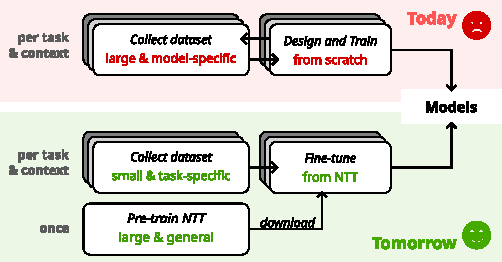
\includegraphics[scale=1.3]{figures/vision}
    \caption{Our vision: Collectively learn general network traffic dynamics \emph{once} and focus on task-specific data collecting and learning  for \emph{many future models?}}
    \label{fig:vision}
\end{figure}

While research shows some generalization in specific networking contexts\cite{jayDeepReinforcementLearning2019}, truly ``generic'' models, which are able to perform well on a wide range of tasks and networks, remain unavailable. This is caused by the fact that we usually do not train on datasets large enough to allow generalization, we only train on task-specific smaller datasets. Sequence modelling for a long time, has been infeasible even with architectures dedicated to sequence modelling, such as recurrent neural networks (RNNs), as they can only handle short sequence and are inefficient to train\cite{factor}. However, a few years ago, a new architecture for sequence modelling was proposed: the \emph{Transformer}\cite{vaswaniAttentionAllYou2017} and this proved to be ground-breaking for sequence modelling. This architecture is designed to train efficiently, enabling learning from massive datasets and unprecedented generalization. In a \emph{pre-training phase}, the transformer learns sequential ``structures'', \eg the structure of a language from a large corpus of texts. Then, in a much quicker \emph{fine-tuning phase}, the final stages of the model are adapted to a specific prediction task (\eg text sentiment analysis). Today, Transformers are among the state-of-the-art in natural language processing (NLP\cite{recentnlp}) and computer vision (CV\cite{cvsurvey}).

The generalization power of the Transformer, stems from its ability to learn ``contextual information'', using context from the neighbouring elements in a sequence, for a given element in the same sequence\cite{devlinBERTPretrainingDeep2019}.\footnote{Consider the word \emph{left} in two different contexts: I \emph{left} my book on the table. Turn \emph{left} at the next crossing. The transformer outputs for the word \emph{left} are different for each sequence as they encode the word's context.}
We can draw parallels between networking and NLP. In isolation, packet metadata (headers, etc.) provides limited insights into the network state, we also need the \emph{context}, \ie which we can get from the recent packet history.\footnote{Increasing latency over history indicates congestion.} Based on these parallel, we propose that a Transformer based architecture can also be design to generalise on network packet data. 

Naively transposing NLP or CV transformers to networking fails, as the fundamental structure and biases\cite{biases} in the data are different. Generalizing on complex interactions in networks is not a trivial problem. We expect the following challenges for our Transformer design.

\begin{itemize}
    \item
          How do we adapt Transformers for learning on networking data?
    \item
          How do we assemble a dataset large and diverse enough to allow useful generalization?
    \item
          Which pre-training task would allow the model to generalize, and how far can we push generalization?
    \item 
    	 How to we scale such a Transformer to arbitrarily large amounts of network data from extremely diverse environments?
\end{itemize}

\section{Overview}
\label{sec:overview}

We present in our thesis, a Network Traffic Transformer (NTT), which servers a first step, to design a Transformer model for learning on network packet data. We outline the following main technical contributions in this thesis:

\begin{itemize}
\item We present the required background on Transformers, which gives directions to our design, in Chapter \ref{cha:background}.
\item We present the detailed architectural design ideas behind our proof-of-concept NTT in Chapter \ref{cha:design}.
\item We present a detailed evaluation on pre-training and fine-tuning our first NTT models in Chapter \ref{cha:evaluation}.
\item We present several future research directions which can be used to improve our NTT in Chapter \ref{cha:outlook}.
\item We summarise our work and provide some concluding remarks in Chapter \ref{cha:summary}.
\item Supplementary technical details and supporting results are presented in Appendix \ref{app:a}, \ref{app:b} and \ref{app:c}. 
\end{itemize}

A part of the work conducted during this thesis has been submitted as the following paper\cite{newhope} to HotNets '22, and hence, we have some parts of the thesis have been built upon work done in writing the paper.

\chapter{Background and Related Work}
\label{cha:background}

A large part of the work undertaken during this project requires a deep understanding on how a particular deep learning architecture, the Transformer works. In this section, we will cover some of the required background and insights drawn from the Transformer architecture which were needed to model and solve our problem of prediction on packet data. We also present adaptations of the Transformer architecture to solve problems in several fields such as NLP/CV and relevant ideas which could be adapted to our tasks.

\section{Background on Transformers}
\label{sec:background}

\subsection{Sequence modelling with attention}
\label{ssec:bgsequence}

Transformers are built around the \emph{attention mechanism}, which maps an input sequence to an output sequence of the same length.
Every output encodes its own information and its context, ie information from related elements in the sequence, regardless of how far they are apart.
The process involves the scalar multiplication of the input feature matrix attention matrix as a dot product operation, which allows the deep neural network to focus on certain parts of the sequence at a time, based on the values of the attention weight matrix. This allows the network to attend to parts of the sequence in parallel, rather than in sequence, which allows highly efficient computation. Also, as the attention weights are learnable parameters for the network, the Transformer over time, learns to choose the best weights which allow optimum learning of structure within the sequence of data.
Computing attention is efficient as all elements in the sequence can be processed in parallel with matrix operations that are highly optimised on most hardware. These properties have made Transformer based neural networks the state-of-the-art solution for solving many sequence modelling tasks. We refer to an excellent illustrated guide to the Transformer here\cite{trans}.


While attention originated as an improvement to Recurrent Neural Networks(RNNs), it was soon realised that the mechanism could replace them entirely.\cite{vaswaniAttentionAllYou2017}
RNNs were the initial state-of-the art deep learning architectures in sequence modelling problems, however they suffer from several issues. Training RNNs is usually limited by one or all of the following problems:
\begin{enumerate}
\item RNNs are not computationally efficient for training long sequences, as they require $n$ sequential operations to learn a sequence, $n$ being the length of the given sequence. This makes the training process extremely slow.
\item RNNs suffer from the problem of \emph{vanishing gradients} \ie as elements in the input need to be processed in a sequence over time, the gradients used by the optimiser\cite{Robbins2007ASA} for the elements at the end of very long sequences, become extremely small and numerically unstable to converge to the desired value.
\item RNNs struggle to learn \emph{long-term dependencies}, \ie learning relations between elements far apart in the sequence is challenging.
\end{enumerate}

We present an excellent summary of the complexities and differences between several deep learning architectures which have attempted to solve the sequence modelling problem in Table \ref{bg:table1}.

\begin{table}[htbp]
\centering
\begin{tabular}{ c   c   c  c  }
\toprule
Layer Type & Complexity   & Sequential   & Maximum \\
& per Layer & Operations & Path Length \\
\midrule
Transformer(Self-Attention) & $O(n^2 \cdot d)$ & $O(1)$ & $O(1)$ \\
Recurrent NN & $O(n \cdot d^2)$ & $O(n)$ & $O(n)$ \\
Convolutional NN & $O(k \cdot n \cdot d^2)$ & $O(1)$ & $O(\log_{k}{n})$\\
Restricted(Self-Attention) & $O(r \cdot n \cdot d)$ & $O(1)$ & $O(n/r)$\\
\bottomrule
\end{tabular}
\caption{Maximum path lengths, per-layer complexity and minimum number of sequential operations
for different layer types. $n$ is the sequence length, $d$ is the representation dimension, $k$ is the kernel
size of convolutions and $r$ the size of the neighbourhood in restricted self-attention.
SOURCE: Original paper\cite{vaswaniAttentionAllYou2017}}
\label{bg:table1}
\end{table}


Augmenting RNNs with attention solves some of these issues\cite{rnnattention},  and replacing them with \emph{Transfomers} has shown to solve all these problems.
The authors propose an architecture for translation tasks that contains:
\begin{itemize}
\item a learnable \emph{embedding} layer mapping words to vectors
\item a \emph{transformer encoder} encoding the input sequence
\item a \emph{transformer decoder} generating an output sequence based on the encoded input
\end{itemize}

Each transformer block alternates between attention and linear layers, ie between encoding context and refining features. The attention mechanism helps learn ``context rich" representations of every element, mapping relevant information from the surrounding elements which surround it and the linear layers help map this learn information into a form useful for downstream prediction. Figure \ref{fig:transformer} shows details of the original Transformer architecture and the functions of its layers.

\begin{figure}[!hbt]
  \begin{center}
    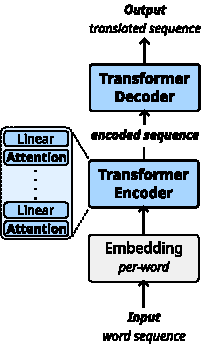
\includegraphics[scale=1.5]{figures/architecture_transformer.pdf}
    \caption{Original Transformer Architecture, Credits: Alexander Dietmüller}
    \label{fig:transformer}
  \end{center}
\end{figure}

\subsection{Pre-training and fine-tuning}
\label{ssec:bgtraining}

Due to the highly efficient and parallelizable nature of Transformers, they can be widely used a variety of tasks based on the principle of \emph{transfer learning}. The most common strategy for that is to use the architecture for two phases, \emph{pre-training} and \emph{fine-tuning}. Inspired by the original Transformers success on the task of language translation, the use of Transformers has become ubiquitous in solving NLP problems. We present one such state of the the art NLP Transformer model, 
called BERT\cite{devlinBERTPretrainingDeep2019}, one of the most widely used transformer models today.
While the original Transformer had both an encoder and decoder with attention, BERT uses only the transformer encoder followed by a small and replaceable decoder. This decoder is usually a set of linear layers and acts as a multilayer perceptron (MLP); and is usually called the 'MLP head' in the deep learning community. The principle of transfer-learning works for BERT as follows:

\begin{itemize}
\item In the first step, BERT is \emph{pre-trained} with a task that requires learning the underlying language structure. Linguists' research has shown that a Masked Language Model is optimal for deep learning models for learning structure in natural languages.\cite{wettigShouldYouMask}
Concretely, a fraction of words in the input sequence is masked out (15\% in the original model), and the decoder is tasked to predict the original words from the encoded input sequence.
BERT is used to generate contextual encodings of, which is only possible due to the bi-directionality of the attention mechanism in BERT. This allows the model to infer the context of the word from both sides in a given sentence, which was not possible earlier when elements in a sequence were only processed in a given order.\footnote{
    BERT is pre-trained from text corpora with several billion words and fine-tuned with $\sim$100 thousand examples per task.
}

\item In the second step, the unique pre-trained model can be fine-tuned to many different tasks by replacing the small decoder with task-specific ones, eg language understanding, question answering, or text generation.
The fine-tuning process involves resumption of learning from the saved weights of the pre-training phase, but for a new task or learning in a new environment. The new model has already learned to encode a general language context and only needs to learn to extract the task-relevant information from this context. This requires far less data compared to starting from scratch and makes the pre-training process faster.

Furthermore, BERTs pre-training step is unsupervised/self-supervised, \ie it requires only ``cheap'' unlabelled data and no labelled signal from the data a target value. As procuring labelled data is harder, this problem is mitigated by having a pre-training phase on ``generic" data and then using 
``expensive'' labeled data, eg for text classification, during the fine-tuning phase. Figure \ref{fig:bert} shows the details of BERT's pre-training and fine-tuning phase.
\end{itemize}

\begin{figure}[!hbt]
  \begin{center}
    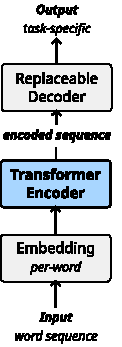
\includegraphics[scale=1.5]{figures/architecture_bert.pdf}
    \caption{Original BERT Architecture, Credits: Alexander Dietmüller}
    \label{fig:bert}
  \end{center}
\end{figure}



Another extremely useful feature of Transformer is its generalization ability, which is  possible due to its highly efficient parallelization during training, which in turn helps transfer of knowledge to a variety of tasks during the process of fine-tuning. The OpenAI GPT-3\cite{brownLanguageModelsAre2020} model that investigates few-shot learning with only a pre-trained model.
As it is just a pre-trained model, it does not outperform fine-tuned models on specific tasks. However, GPT-3 delivers impressive performance on various tasks, including translation, determining the sentiment of tweets, or generating completely novel text. As per requirement, it can also be fine-tuned on specific tasks, which showcases further, the generalization power of transformers.


\subsection{Vision transformers}
\label{ssec:bgvit}

Following their success in NLP, the use of Transformers were explored as a possibility to learn structural information in other kinds of data. One such field where they gained a lot of traction in in the field of CV.
However adapting the use of Transformers to vision tasks came with a few major challenges: 
\begin{itemize}
\item Image data does not have a natural sequence, as they are a spatial collection of pixels.
\item Learning encodings at the pixel level for a large number of images, proved to be too fine-grained to scale to big datasets.
\item The Masked Language Model theory couldn't be efficiently transferred to the context of learning structure in images, as the relationship between the units (pixels) does not follow the same logic as in natural languages.
\end{itemize}

To solve this problems, the authors of the Vision Transformer(ViT)\cite{dosovitskiyImageWorth16x162021}, came up with multiple ideas to solve each of these problems, in order to have the data in a form, on which a Transformer could be efficiently trained.
\begin{itemize}
\item \emph{Serialize and aggregate the data: } As image data does not have a natural sequence structure, such a structure was artificially introduced. Every image was split at the pixel level and aggregated into patches of dimension 16$\times$16 and each of these patches became a member of the new input ``sequence". As Transformers scale quadratically with increasing sequence size \ref{bg:table1}, this also solved the problem of efficiency and that encodings at the pixel level are too fine-grained to be useful. The embedding and transformer layers were then applied to the resulting sequence of patches, using an architecture similar to BERT.
\item \emph{Domain Specific Pre-training: } At the heart, most CV problems have very similar training and inference objectives, one of the most common being image classification, which makes most of the vision tasks similar in objective, differing only in environment. This made classification a much more suited task for image data pre-training as opposed to masking and reconstruction. This was exploited by the ViT and both the pre-training and fine-tuning was done with the objective of classification, with only a change in environment between the stages. This also meant that understanding structure in image data, not only required information from the neighbouring patches but also from the whole image, which was possible by using all the encoded patches for classification. We present the details of ViT's pre-training and fine-tuning in Figure \ref{fig:vit}.
\end{itemize}

\begin{figure}[!hbt]
  \begin{center}
    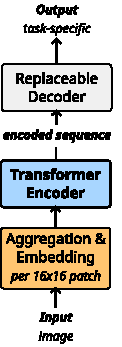
\includegraphics[scale=1.5]{figures/architecture_vit.pdf}
    \caption{Original ViT Architecture, Credits: Alexander Dietmüller}
    \label{fig:vit}
  \end{center}
\end{figure}


Finally, ViT's authors also observe that domain-specific architectures that implicitly encode structure, like convolutional networks (CNNs) work extremely well for image datasets and  actually result in better performance on small datasets. However, given enough pre-training data, learning sequences with attention beats architectures that encode structure implicitly, making the process a tradeoff between the utility and the amount of resources required for pre-training. Later research in the field has also shown advancements in vision based transformers which use a masked reconstruction approach\cite{heMaskedAutoencodersAre2021}, such details however are beyond the scope of this section. 


\section{Related Work}
\label{sec:related_work}

The problem of learning networks dynamics from packet data has been deemed a complex ``lost cause'',  and not a lot of the research community has made much direct effort in this direction. The idea of using large pre-trained machine learning models to learn from abstract network traces, has thus not been explored much. However, application specific adaptions of ML architectures have been used with varying amount of success on network data, and we present some of these efforts and successes here, which helped provide direction to our own ideas and thoughts for this project.

In MimicNet\cite{zhangMimicNetFastPerformance2021}, the authors  show that they can provide users with the familiar abstraction of a packet-level simulation for a portion of the network while leveraging redundancy and recent advances in machine learning to quickly and accurately approximate portions of the network that are not directly visible. In Puffer\cite{puffer},  they use supervised learning in situ, with data from the real deployment environment, to train a probabilistic predictor of upcoming chunk transmission times for video streaming. The authors of Aurora\cite{jayDeepReinforcementLearning2019} show that casting congestion control as a reinforcement learning (RL) problem enables training deep network policies that capture intricate patterns in data traffic and network conditions but also claim that fairness, safety, and generalization, are not trivial to address within conventional RL formalism. Pensieve\cite{maoNeuralAdaptiveVideo2017} trains a neural network model that selects bitrates for future video chunks based on observations collected by client video players and  it learns to make ABR decisions solely through observations of the resulting performance of past decisions. Finally, in NeuroPlan\cite{planning} they propose to use a graph neural network (GNN) combined with a novel domain-specific node-link transformation for state encoding and following that, leverage a two-stage hybrid approach that first uses deep RL to prune the search space and then uses an ILP solver to find the optimal solution for the network planning problem.






\chapter{Design}
\label{cha:design}

\section{Dataset Generation}
\label{sec:ns3}

Note: Will decide later if we want to move this to a new chapter or not.

\section{Network Traffic Transformer (NTT)}
\label{sec:ntt}

This chapter describes your work in detail and is normally the longest chapter.
You can also create multiple chapters describing your work.

It is often useful to format your text with \textbf{bold} or \textit{italic}
\emph{words}. In addition, it can be helpful to format text as verbatim:

\begin{verbatim}
Verbatim representation
    of     my
text.
\end{verbatim}

Finally, you can also add a mathematical formula inline $a^2 + b^2 = c^2$ or in
its own block:

\begin{equation}
    \cos (2\theta) = \cos^2 \theta - \sin^2 \theta
\end{equation}


\chapter{Evaluation}
\label{cha:evaluation}

Another important chapter is the evaluation which should clearly describe the
experiments you performed (setup, number of measurements, \dots), show the
results you achieved in figures and/or tables and discuss and compare the
results.

\section{Fine-tuning Dataset}
\label{eval:ft}

\section{Experimental Results}
\label{eval:res}
\chapter{Outlook}
\label{cha:outlook}

What are consequences of your work? Do you see possibilities for future work?
\chapter{Summary}
\label{cha:summary}

Give a final, short summary of your work.


\clearpage

\addcontentsline{toc}{chapter}{References}

\bibliographystyle{acm}
\bibliography{refs}

\clearpage
\begin{appendices}

\pagenumbering{Roman}

\chapter{NTT training details}
\label{app:a}

We present here further specifics about the choices made during pre-training and fine-tuning our NTT architecture. We also present the common hyper-parameters used for both. In the scope of our project, we do not perform a search to find the best performing hyper-parameters. Our objective is to explore what can be learnt, and not to achieve state-of-the-art results. The hyper-parameters for us are chosen based on Transformers trained in other domains, and with some tweaking, work reasonably well for our use case.

We implement our NTT in Python, using the PyTorch\cite{pytorch} and PyTorch Lightning\cite{pytorchlit} libraries. We implement our NTT in a Debian $10$ environment. For our training process, we use NVIDIA\textsuperscript{\textregistered} Titan Xp GPUs, with $12$ GB of GPU memory. For pre-training and fine-tuning on the full datasets, we use 2 GPUs with PyTorch's DataParallel implementation. For pre-processing our data, generating our input sliding window sequences and converting our data into training, validation and test batches, we use $4$, Intel\textsuperscript{\textregistered} $2.40$ GHz Dual Tetrakaideca-Core Xeon E5-2680 v4 CPUs and   between $60-80$ GB of RAM. 

\begin{table}[htbp]
\centering
\begin{tabular}{ l   c  }
\toprule
\emph{Hyper-parameter} & Value  \\
                                                       
\midrule
 Learning rate                                         &     $1\times10^{-4}$           \\
 Weight decay					  &       $1\times10^{-5}$          \\
 \# of attention heads 			  &          $8$      \\
 \# of Transformer layers			  &          $6$        \\
 Batch size 			  		&            $64$      \\
 Dropout prob.					&            $0.2$   \\
 Pkt embedding dim.			&                   $120$     \\
    
\bottomrule

\end{tabular}
\caption{Hyper-parameters for NTT training}
\label{app:table1}
\end{table}

We refer to Table \ref{app:table1} to discuss our training hyper-parameters. The number of attention heads refers to the number of attention matrices used inside the Transformer encoder layers, which are processed in parallel. In our NTT architecture (Figure \ref{fig:ntt}), we have $691K$ trainable parameters from the embedding and aggregation layers, $3.3M$ trainable parameters from the Transformer encoder layers and $163K$ trainable parameters from linear layers in the decoder. We use $4$ linear layers in the decoder, with activation and layer-weight normalisation\cite{layernorm} between each linear layer.  We also use a layer-weight normalisation layer, as a pre-normalising layer, on the output of the embedding and aggregation. During training, we use a dropout probability\cite{dropout} of $0.2$ and a weight decay\cite{weightdecay} over the weights (not biases), in order to prevent overfitting. We use a batch size of $64$, to reduce the noise during our training process.

We use the ADAM\cite{adam} optimiser with $\beta_1=0.9$, $\beta_2=0.98$ and $\epsilon=1\times10^{-9}$, for our training and the Huber loss\cite{huber} function for training loss (\ref{eq:huber}), as it is not super-sensitive to outliers but neither ignores their effects entirely. The loss function is computed on the residual \ie the difference between the observed  and predicted values, $y$ and $f(x)$ respectively.
\begin{equation}
L_\delta(y, f(x))=
    \begin{cases}
        \frac{1}{2}(y - f(x))^2 & \text{for } \lvert y - f(x) \rvert \leq \delta, \\
        \delta  \cdot (\lvert y - f(x) \rvert - \frac{1}{2}\delta) & \text{otherwise}
    \end{cases}
\label{eq:huber}
\end{equation}

We use a warm-up scheduler over our base learning rate (lr) of  $1\times10^{-4}$, as mentioned in the original Transformer paper\cite{vaswaniAttentionAllYou2017}. We present the governing equation for that as (\ref {eq:lr})

\begin{equation}
lr = d_{model}^{-0.5} \cdot \min{(step\_num^{-0.5}, warmup\_steps^{-0.5})}
\label{eq:lr}
\end{equation}

This corresponds to increasing the learning rate linearly for the first \emph{warmup\_steps} training steps, and decreasing it thereafter proportionally to the inverse square root of the step number. We used $warmup\_steps = 4000$ and our pre-training data has ${\sim}17K$ steps, and our $d_{model}$ is $120$.


\chapter{Learning with multiple decoders}
\label{app:b}

In Section \ref{ssec:impptt}, we evaluated the idea of masking different positions in the input sequence, in order to improve the pre-training phase of the NTT.  During this, we realised that with a variable masking approach, it is not always feasible to have a single set of linear layers to effectively act a combined MLP decoder, across all levels of aggregation. We present some further results on using different instances of identical MLP decoders, for different levels of aggregation, which are due to selecting the packet delays to be masked in different ways for pre-training. We summarise our findings in Table \ref{app:table2}

\begin{table}[htbp]
\centering
\begin{tabular}{ l   c  }
\toprule
\emph{all values $\times10^{-3}$} & Pre-training \\
(Masking + MLP instance) & (Delay)  \\
                                                       
\midrule
\em{NTT: Chosen mask}                                              & 		 	 \\
\smallindent From encoded states + 1 MLP decoder                                         &      0.063         \\
\smallindent From encoded states + 3 MLP decoders                                         &     0.070          \\
\smallindent From aggregation levels + 1 MLP decoder  					&     1.31          \\
\smallindent  From aggregation levels + 3 MLP decoders  					&     0.087          \\
 
    
\bottomrule

\end{tabular}
\caption{MSE on delay prediction across NTT with multiple instances of linear MLP decoders}
\label{app:table2}
\end{table}

Based on our experiments, it is evident that we will need different instances of MLP decoders, when we mask across different levels of aggregation, with varying frequency of masking. In the case, where we choose from \emph{the encoded states}, we only choose the packets which are aggregated twice $1/48$ of the times, and we mainly choose the non-aggregated packets ($32/48$ of the times). In this scenario, it doesn't hurt the performance even if we use a single set of linear layers to extract the learnt behaviour across levels of aggregation, as most of the times, the non-aggregated packets are chosen. In this case, using a single MLP decoder vs using $3$ MLP decoders for learning has very similar performance.

When we choose from \emph{aggregation levels}, the situation is very different as we mask $1/2$ the packet delays, which are aggregated twice, $1/3$ of the times. In this scenario, a single MLP decoder cannot effectively learn across levels of aggregation, all of which are chosen frequently and in this case, using multiple MLP decoders, helps the learning process. 

Based on the fact that different aggregation schemes may be used in future version of the NTT, different numbers of MLP decoders will be needed. One can certainly be sure that, with increasing complexity and aggregation, more complexity will also be required in the decoder architecture, to learn newer kinds of information.


\end{appendices}

\end{document}
